\documentclass[tikz,border=2pt]{standalone}
\usepackage{amsmath}
\usepackage{pgfplots}
\pgfplotsset{compat=1.18}

\begin{document}
% All antiderivatives of f(x)=x are F(x)=x^2/2+C: one family of vertically shifted curves,
% all with the same slope f(x) at each x.
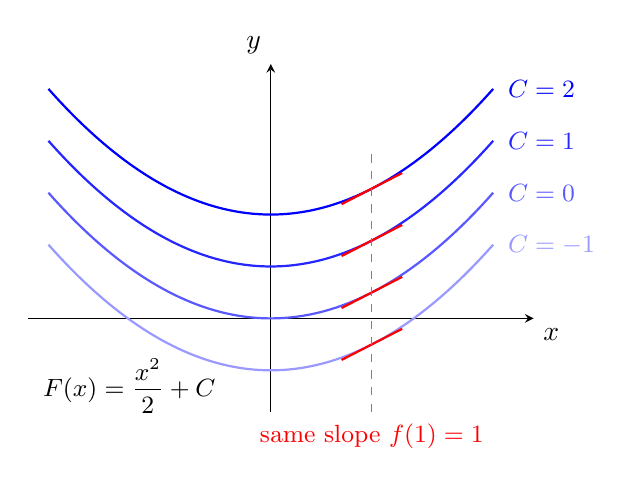
\begin{tikzpicture}
	\begin{axis}[
		axis lines=middle,
		xmin=-2.4, xmax=2.6,
		ymin=-1.8, ymax=4.9,
		xtick=\empty, ytick=\empty,
		xlabel={$x$}, ylabel={$y$},
		xlabel style={below right}, ylabel style={above left},
		samples=80, smooth, clip=false,
		width=8cm, height=6cm
		]
		\addplot[blue!40, thick, domain=-2.2:2.2] {x^2/2-1};
		\addplot[blue!65, thick, domain=-2.2:2.2] {x^2/2};
		\addplot[blue!85, thick, domain=-2.2:2.2] {x^2/2+1};
		\addplot[blue, thick, domain=-2.2:2.2] {x^2/2+2};
		\node[blue!40, anchor=west, font=\small] at (axis cs:2.25,1.42) {$C=-1$};
		\node[blue!65, anchor=west, font=\small] at (axis cs:2.25,2.42) {$C=0$};
		\node[blue!85, anchor=west, font=\small] at (axis cs:2.25,3.42) {$C=1$};
		\node[blue, anchor=west, font=\small] at (axis cs:2.25,4.42) {$C=2$};
		% equal slopes at x=1
		\draw[red, thick] (axis cs:0.7,-0.8) -- (axis cs:1.3,-0.2);
		\draw[red, thick] (axis cs:0.7,0.2) -- (axis cs:1.3,0.8);
		\draw[red, thick] (axis cs:0.7,1.2) -- (axis cs:1.3,1.8);
		\draw[red, thick] (axis cs:0.7,2.2) -- (axis cs:1.3,2.8);
		\draw[dashed, gray] (axis cs:1,-1.8) -- (axis cs:1,3.2);
		\node[red, anchor=north, font=\small] at (axis cs:1,-1.85) {same slope $f(1)=1$};
		\node[anchor=west, font=\small] at (axis cs:-2.35,-1.3) {$F(x)=\dfrac{x^2}{2}+C$};
	\end{axis}
\end{tikzpicture}
\end{document}
